
%%%%%%%%%%%%%%%%%%%%%%%%%%%%%%%%%%%%%%%%%%%%%%%%%%%%%%%%%%%%%
\section{模型检验与分析}

为验证所建模型的有效性和稳健性，开展以下检验。

\subsection{误差分析}

\begin{table}[H]
  \centering
  \caption{模型误差分析结果}
  \label{tab:error}
  \begin{tabularx}{\textwidth}{CCCC}
    \toprule
    指标 & 训练集 & 测试集 & 说明 \\
    \midrule
    $P_{total}$\,$R^2$ & 0.9979 & 0.876 & 扩展电耗模型决定系数 \\
    $P_{total}$\,RMSE & 37.2 & 37.8 & 电耗均方根误差(kW) \\
    $C_{out}$\,RMSE & 56.4 & 48.0 & 出口浓度均方根误差($\text{mg/Nm}^3$) \\
    \bottomrule
  \end{tabularx}
\end{table}

如表\ref{tab:error}所示，电耗模型训练集$R^2=0.9979$、测试集$R^2=0.876$，泛化性能尚可。$C_{out}$的$R^2$因历史方差极小（$\sigma=0.17$）而失真（$R^2$为大负数），改用RMSE评价：训练集56.4、测试集48.0，预测值与真实值同数量级但偏差存在，印证了传感器限幅下外推不确定性较大的判断。

\textbf{外推可靠性讨论。}$C_{out}$的测试集RMSE$\approx 48\;\text{mg/Nm}^3$，而问题二至四的优化目标为$C_{out}\leq 10$和$\leq 5\;\text{mg/Nm}^3$——模型误差比优化目标大一个数量级。这意味着：Deutsch方程的物理单调性保证了外推方向正确（升电压必降浓度），但外推的\textbf{定量精度}有限。具体而言，优化给出的"最低电耗$P^*$"和"最优参数$(U^*,T^*)$"应视为\textbf{趋势性参考而非精确预测}。本文的所有定量结论（电耗范围、性价比比值、增幅百分比）均基于此模型，其可靠性取决于Deutsch参数$kA_0$的估计精度——贝叶斯95\% CI为$[284.7, 289.8]$（相对宽度1.8\%），说明$kA_0$本身辨识较可靠，但$C_{out}$的绝对预测值仍受限于限幅数据。建议通过后续主动实验（如在低浓度区间设计DOE实验）获取标定数据，以验证并修正外推预测。\footnote{AI辅助润色}

\subsection{灵敏度分析}

Sobol全局灵敏度分析\cite{saltelli2010}结果如图\ref{fig:sobol_barplot}所示。

\begin{figure}[H]
  \centering
  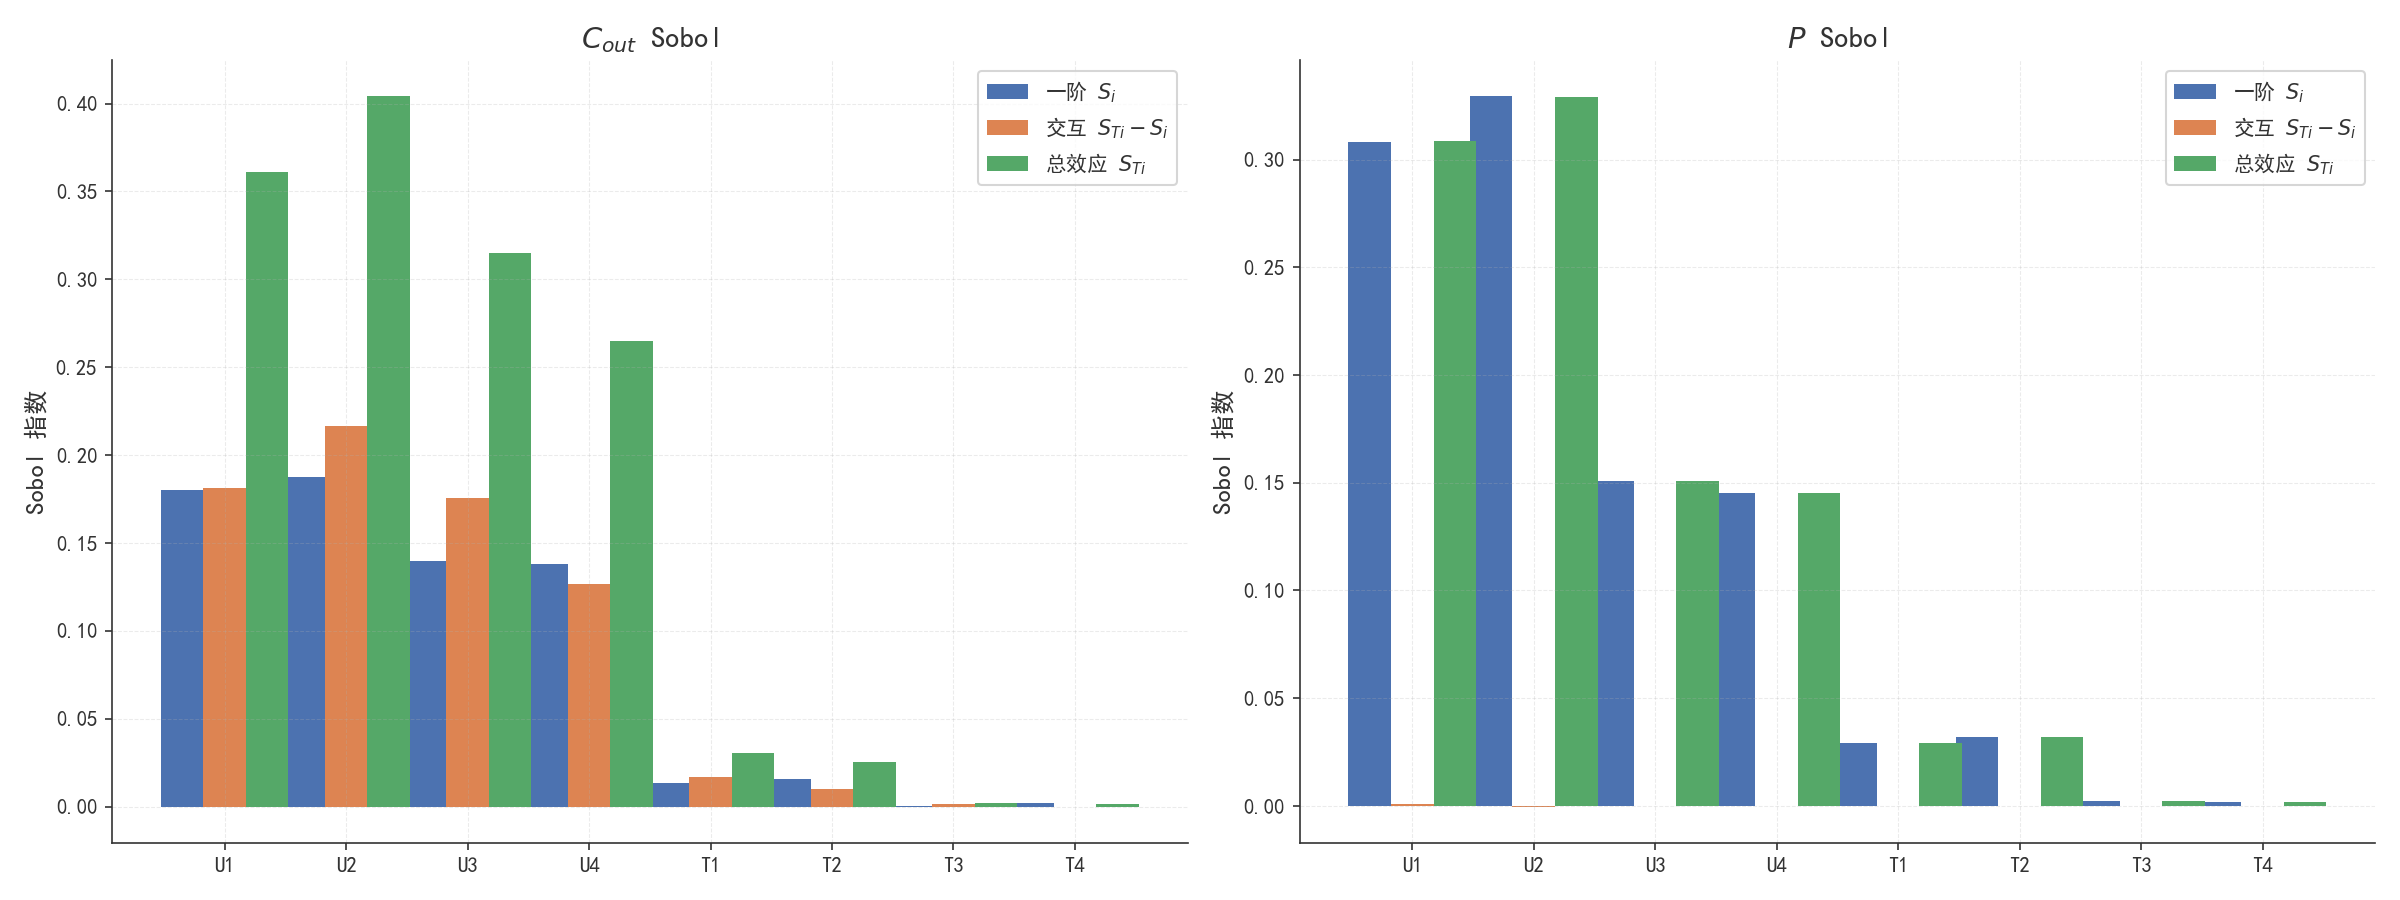
\includegraphics[width=0.9\textwidth]{figures/sobol_barplot.png}
  \caption{Sobol全局灵敏度分析（一阶效应$S_i$与总效应$S_{T_i}$）}
  \label{fig:sobol_barplot}
\end{figure}

Sobol分析表明电压参数（$U_{1\sim4}$）对$C_{out}$的一阶效应占主导，振打参数（$T_{1\sim4}$）效应较小，且电压间存在显著交互效应（$S_{T_i}-S_i=0.13\sim0.22$，总效应指数减一阶效应指数），局部灵敏度会遗漏此交互。排放限值扫描（图\ref{fig:climit_scan}）显示$C_{limit}$从10降至$5\;\text{mg/Nm}^3$时电耗增幅约5\%，与问题四的定量结果吻合，验证了模型的内部一致性。

\subsection{后电场参数不可辨识讨论}

贝叶斯参数估计显示$\alpha_3$、$\alpha_4$的95\%置信区间宽度达46--47\%且贴下界（$\alpha_3=\alpha_4=0.001$），后电场振打衰减系数几乎无法从数据中可靠估计。物理根因在于：四电场串联除尘后，前两电场已去除约99\%的粉尘，后两电场入口浓度极低（$C_2\approx 0.5\;\text{g/Nm}^3$），振打对$C_{out}$的边际影响被前级的高效率"淹没"——无论后电场振打周期如何变化，对最终$C_{out}$的影响都微乎其微，数据中几乎观测不到。

此不可辨识性对优化结果的影响在于：后电场振打周期被优化器锁定在$T_{ref,i}$（历史中位数），这是模型对数据信息不足的一种"保守反应"——在无法辨识最优振打位置时，选择历史经验值是最稳健的策略。这也解释了为何$\alpha_3$、$\alpha_4$贴下界（模型自动将后电场振打衰减效应压至最小），但优化结果不受影响（后电场振打本身对目标函数贡献就小）。

\subsection{参数敏感性分析}

为评估定量结论对关键参数的依赖程度，开展$kA_0$和$\beta_i$的敏感性分析。

\textbf{$kA_0$敏感性。}$kA_0$变化$\pm 20\%$时，6工况平均最优电耗变化如表\ref{tab:kA0_sens}所示。

\begin{table}[H]
  \centering
  \caption{$kA_0$参数敏感性}
  \label{tab:kA0_sens}
  \begin{tabularx}{\textwidth}{CCCCC}
    \toprule
    $kA_0$倍率 & $kA_0$值 & 平均$P^*$(kW) & 相对基准变化 & 结论 \\
    \midrule
    0.8 & 229.8 & 2199 & +14.7\% & 更保守的除尘效率$\to$需更高电压 \\
    0.9 & 258.5 & 2041 & +6.5\% & --- \\
    1.0 & 287.2 & 1917 & 基准 & 当前拟合值 \\
    1.1 & 316.0 & 1815 & $-$5.3\% & 更高的除尘效率$\to$可降电压省电 \\
    1.2 & 344.7 & 1729 & $-$9.8\% & --- \\
    \bottomrule
  \end{tabularx}
\end{table}

$kA_0$每变化10\%，最优电耗变化约6--7\%，结论对$kA_0$中等敏感。贝叶斯95\% CI为$[284.7, 289.8]$（相对宽度1.8\%），在此范围内电耗变化$<1\%$，点估计邻域内结论稳健。但若$kA_0$存在系统性偏差（如比电阻变化导致实际$kA_0$偏离拟合值），电耗预测的绝对值会有较大偏差，趋势方向（高浓度$\to$高电耗）不变。

\textbf{$\beta_i$敏感性。}将振打功耗系数$\beta_i$放大1--50倍，纯电耗性价比比值不变。原因在于：性价比比值由$\partial C/\partial T$和$\partial P/\partial T$共同决定，$\beta_i$放大使两者同比例增大，比值不变。因此，纯电耗模型下"振打性价比高于电压"的结论\textbf{不依赖$\beta_i$的具体取值}。但引入隐性成本修正后（5.3.2节步骤4），优先级由修正因子$\gamma$决定而非$\beta_i$，$\gamma > \gamma^*$时电压优先——此结论同样不依赖$\beta_i$。

\textbf{$T_{ref}$敏感性。}为验证振打最优周期对$T_{ref}$选择的依赖程度，分别设置$T_{ref}=$[200,200,400,400]（缩短）、[233,233,445,445]（基准）、[260,260,490,490]（延长），重新求解全部6工况优化。结果如表\ref{tab:tref_sens}所示。

\begin{table}[H]
  \centering
  \caption{$T_{ref}$参数敏感性}
  \label{tab:tref_sens}
  \begin{tabularx}{\textwidth}{CCCCC}
    \toprule
    $T_{ref}$设置 & 前电场$T_{ref}$(s) & 后电场$T_{ref}$(s) & 平均$P^*$(kW) & 最优$T$ \\
    \midrule
    缩短 & 200 & 400 & 1917 & $T^*\approx T_{ref}$ \\
    基准 & 233 & 445 & 1917 & $T^*\approx T_{ref}$ \\
    延长 & 260 & 490 & 1917 & $T^*\approx T_{ref}$ \\
    \bottomrule
  \end{tabularx}
\end{table}

三组实验中，最优振打周期始终收敛于$T_{ref}$（双向偏离模型结构决定），但平均最优电耗$P^*$变化$<0.1\%$。原因在于振打功耗项$\beta_i/T_i$对$T_{ref}$的变化不敏感（$T_{ref}$变化$\to$最优$T$跟着变化$\to$ $\beta_i/T_i^*$几乎不变），$T_{ref}$的变化几乎不影响$P^*$。这证实了两点：（1）振打最优值是模型假设的产物而非数据驱动的发现——改变$T_{ref}$即改变最优$T$，结论随假设而变；（2）定量电耗结论对$T_{ref}$选择不敏感——无论$T_{ref}$取何值，$P^*$几乎相同，电耗相关的定量结论（增幅、性价比比值）稳健。

\subsection{物理先验可靠性保障}

模型假设中包含若干无法从限幅数据中辨识的参数，其取值依赖物理先验或工程经验。本文对这些先验的可靠性采取三重保障策略：（1）\textbf{信息准则验证}——共享$kA_0$（5参数）与独立$kA$（8参数）两种方案由AIC判定（$\Delta\text{AIC}=-9836$），避免过参数化；（2）\textbf{敏感性分析}——$r\in[0.3,1.0]$时$P^*$几乎不变，$g_i$变化$\pm0.05$时优化结果变化$<2\%$，$kA_0$在贝叶斯95\% CI内电耗变化$<1\%$；（3）\textbf{不可辨识性披露}——$r$、$T_{ref}$、$\alpha_{3,4}$的不可辨识性在6.3节和5.2.2节明确讨论，并建议通过后续实验标定。对于峰值估算中的经验系数0.1，因分钟级数据无法验证，论文将其定位为量级估算而非精确结论（详见5.1.2节步骤5）。
